%! Author = Ryan Coslove (rmc326)
%! Due Date = 11/15/2021

\documentclass{article}

\setlength{\headsep}{0.75 in}
\setlength{\parindent}{0 in}
\setlength{\parskip}{0.1 in}

%=====================================================
% Add PACKAGES Here (You typically would not need to):
%=====================================================

\usepackage{xcolor}
\usepackage[margin=1in]{geometry}
\usepackage{amsmath,amsthm,amssymb}
\usepackage{fancyhdr}
\usepackage{enumitem}
\usepackage{algorithm}
\usepackage{algpseudocode}
\usepackage{graphicx}
\usepackage{xspace}
\usepackage{subcaption}

%=====================================================
% Ignore This Part (But Do NOT Delete It:)
%=====================================================

\theoremstyle{definition}
\newtheorem{problem}{Problem}
\def\fline{\rule{0.75\linewidth}{0.5pt}}
\newcommand{\finishline}{\begin{center}\fline\end{center}}
\newtheorem*{solution*}{Solution}
\newenvironment{solution}{\begin{solution*}}{{\finishline} \end{solution*}}
\newcommand{\thisdate}{November 15, 2021}
\newcommand{\thissemester}{\textbf{Rutgers: Fall 2021}}
\newcommand{\thiscourse}{CS 440: Intro to AI} 
\newcommand{\thishomework}{Number} 
\newcommand{\thisname}{Name} 

\headheight 40pt              
\headsep 10pt
\pagestyle{fancy}

\newcommand{\thisheading}{
   \noindent
   \begin{center}
   \framebox{
      \vbox{\vspace{2mm}
    \hbox to 6.28in { \textbf{\thiscourse \hfill \thissemester} }
       \vspace{4mm}
       \hbox to 6.28in { {\Large \hfill Midterm Exam\hfill} }
       \vspace{2mm}
         \hbox to 6.28in { { \hfill \thisdate  \hfill} }
       \vspace{2mm}
       \hbox to 6.28in {{Name: \thisname \hfill}}
      \vspace{2mm}}
      }
   \end{center}
   \bigskip
}

%=====================================================
% Some useful MACROS (you can define your own in the same exact way also)
%=====================================================


\newcommand{\ceil}[1]{{\left\lceil{#1}\right\rceil}}
\newcommand{\floor}[1]{{\left\lfloor{#1}\right\rfloor}}
\newcommand{\prob}[1]{\Pr\paren{#1}}
\newcommand{\expect}[1]{\Exp\bracket{#1}}
\newcommand{\var}[1]{\textnormal{Var}\bracket{#1}}
\newcommand{\set}[1]{\ensuremath{\left\{ #1 \right\}}}
\newcommand{\poly}{\mbox{\rm poly}}


%=====================================================
% Fill Out This Part With Your Own Information:
%=====================================================
\renewcommand{\thisname}{Ryan Coslove (rmc326)} % Enter your name here



\begin{document}

\thisheading
\vspace{-0.75cm}


\begin{problem} %problem 1
	

\end{problem}

\begin{solution}
	\item  1a.)

	\item BFS: A, B, C, D, E, F, G, H, Z
		\begin{figure}[h!]
			\centering
			\IfFileExists{1aBFS.png}{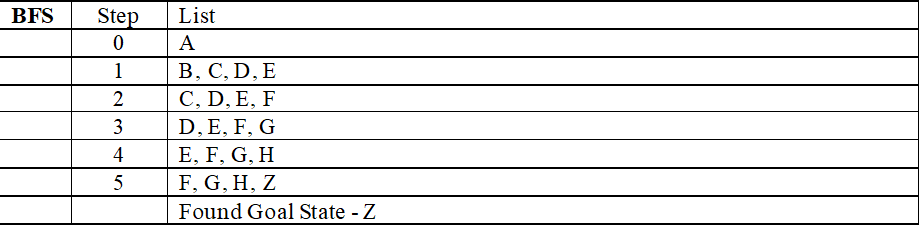
\includegraphics[width=0.9\textwidth]{1aBFS.png}}
		 
		\end{figure}

	\item DFS: A, B, C, D, E, F, G, H, Z
		\begin{figure}[h!]
			\centering
			\IfFileExists{1aDFS.png}{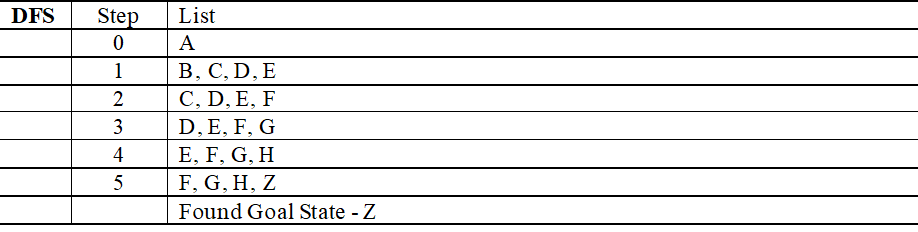
\includegraphics[width=0.9\textwidth]{1aDFS.png}}
		 
		\end{figure}
	\item IDS: A, B, F, I, G, C, A, D, H, J, K, Z
		\begin{figure}[h!]
			\centering
			\IfFileExists{1aIDS.png}{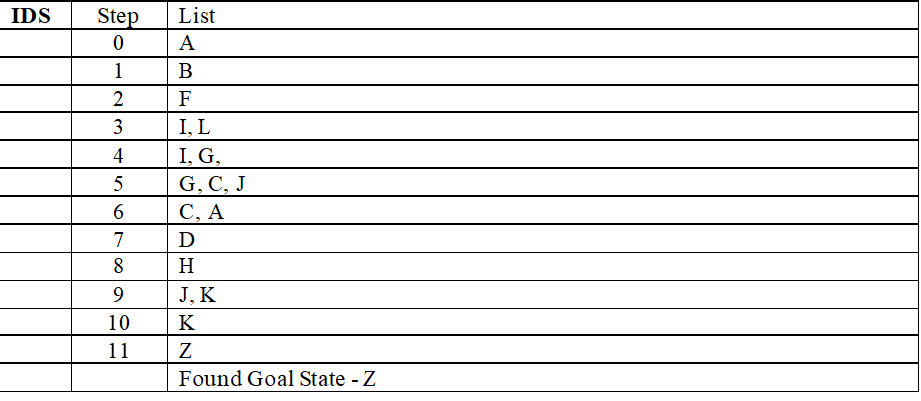
\includegraphics[width=0.9\textwidth]{1aIDS.png}}
		 
		\end{figure}

	\begin{newpage}
	\end{newpage}

	\item A*: A, B, F, L, Z
		\begin{figure}[h!]
			\centering
			\IfFileExists{1aA.png}{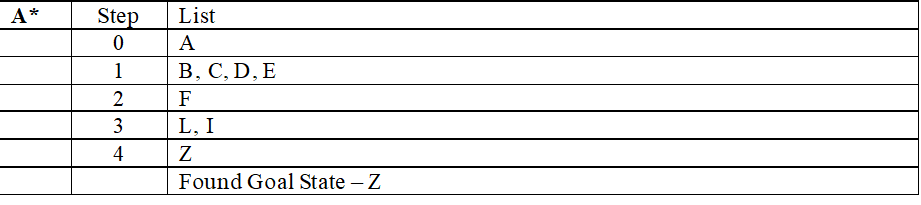
\includegraphics[width=0.9\textwidth]{1aA.png}}
		 
		\end{figure}

	\item 1b.) 
	
	\item A* did find the optimal path. It took the least amount of steps/iterations to find Z because from A, BCDE all had values of 4, so alphabetically we choose B. Then we go to F. The lowest heuristic value from F was L. Then L leads to Z. BFS and DFS took the same amount of steps, each using uniform cost and alphabet as the tiebreaker. IDS took the most steps and was the least optimal path. 

	\item 1c.) 
	\item Yes all methods found a solution using graph-search. All successfuly found goal node Z. A* was the most optimal, IDS was the least optimal. 


\end{solution}

\begin{problem} %problem 2
	
\end{problem}

\begin{solution}
	\item  2a.) 
		\begin{figure}[h!]
			\centering
			\IfFileExists{2a.png}{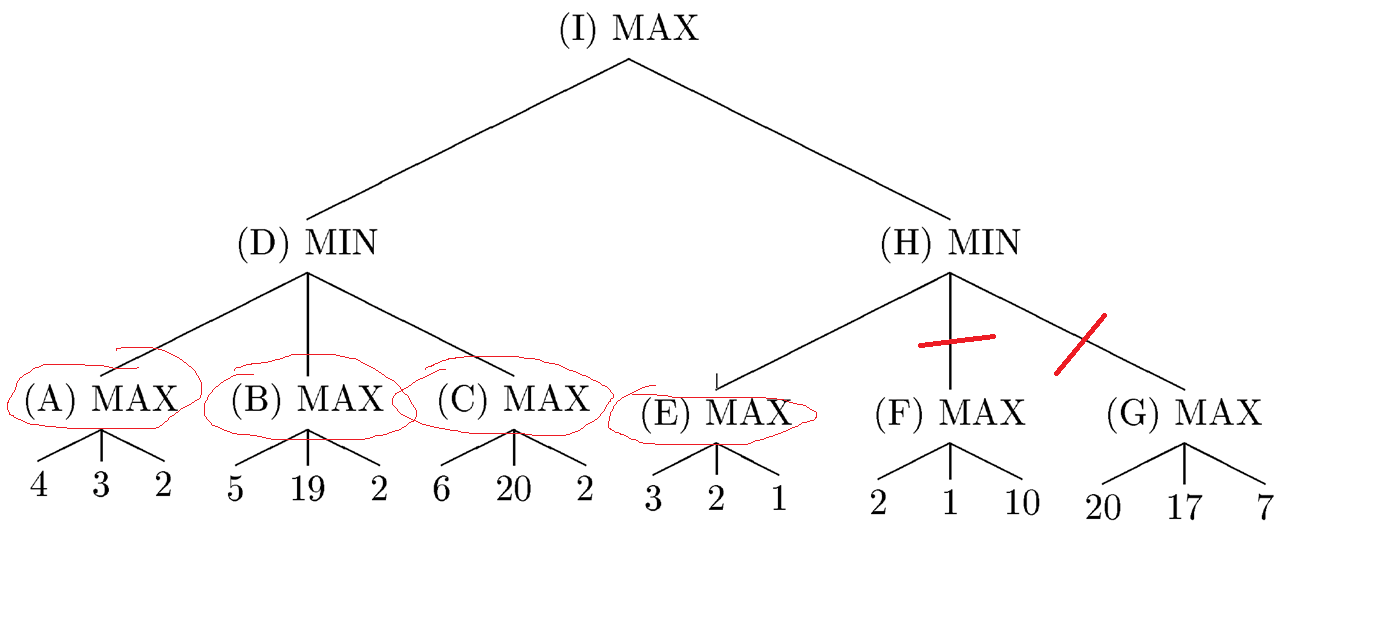
\includegraphics[width=0.9\textwidth]{2a.png}}
		 
		\end{figure}

	\begin{newpage}
	\end{newpage}

	\item 2b.) MAX will move to node D. This is because the MAX of ABC are 4, 19, and 20, respectively. This will return 4 as the MIN for D. The MAX of EFG are 3, 10, 20, respectively. This will return 3 as the MIN of H. So the MAX will choose node D because $4 > 3$ and D $>$ H.

	\item 2c.) The MAX of C is 20. The MAX of G is also 20. So for (D) MIN = 20 and (H) MIN = 20. Given that both MAX values are equal, it does not matter if MAX goes to D or H as its first move.  
	
\end{solution}

\begin{problem} %problem 3

\end{problem}

\begin{solution}
	\item  3a.) 
		\begin{figure}[h!]
			\centering
			\IfFileExists{3a.png}{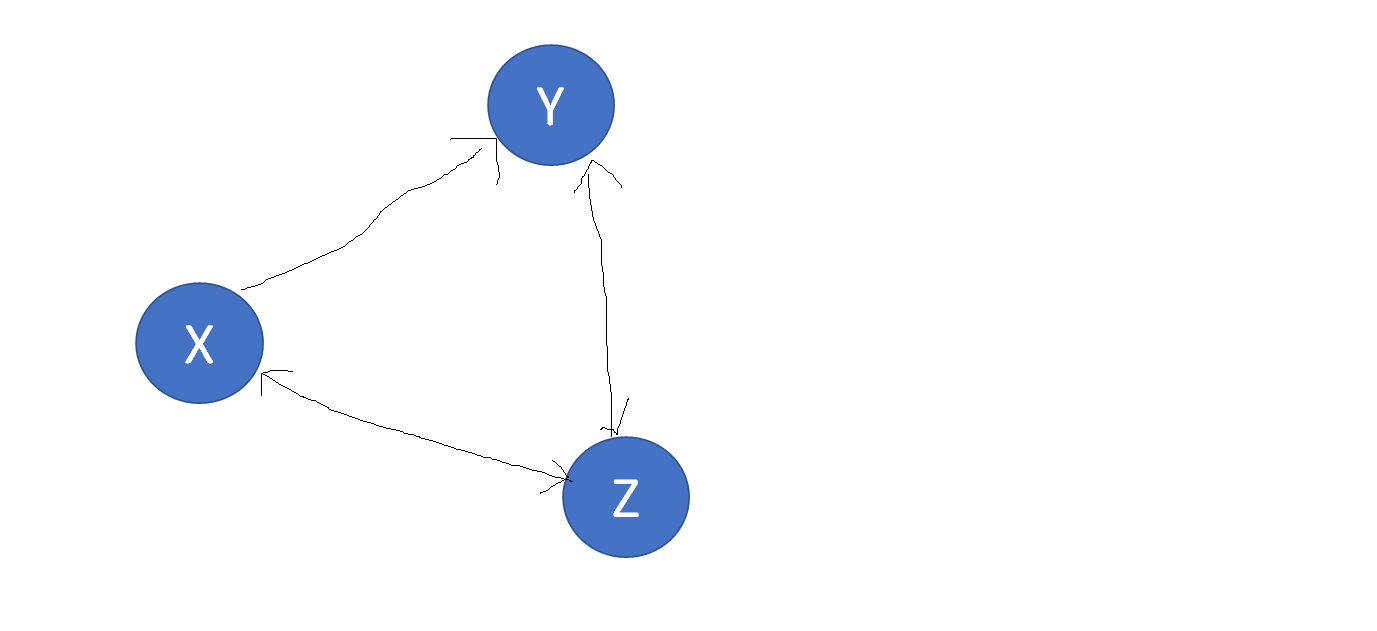
\includegraphics[width=0.9\textwidth]{3a.png}}
		 
		\end{figure}

	\begin{newpage}
	\end{newpage}

	\item 3b.)
		\begin{figure}[h!]
			\centering
			\IfFileExists{3b.png}{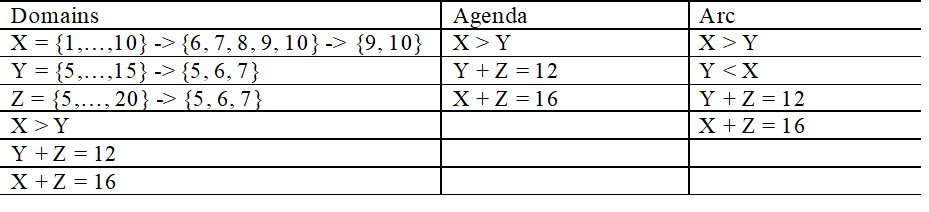
\includegraphics[width=0.9\textwidth]{3b.png}}
		 
		\end{figure}

	
\end{solution}

\begin{problem} %problem 4
	

\end{problem}

\begin{solution}
	\item  Most Constrained Variable: In the search tree, we alternate between choosing variables and choosing values for the variables. At the stage where we choose a variable, we break the search and backtrack if we find one variable that cannot be satisfied. Finding only one such variable is sufficient to say that something was wrong earlier, and we go up in the search to try other assignments. Therefore, we want to fail quickly, which will save us the trouble of trying many variables before finding the one that fails.

	\item Least Constraining Value: Once we choose a variable, we have to try all the possible values before we can say that it failed. Therefore, we will be only choosing time with values that fail (since we will still have to check the remaining values). But if we succeed, the search stops and we don't have to try the remaining values. 
	
\end{solution}



\end{document}